\chapter{Appendix}
\label{chap:appendix}

\section{Replication Code and Classification dataset}

All code to replicate the results as well as all enrichment data classifying the samples of intermediaries can be found here on my GitHub. \href{https://github.com/OscarAdserballe/topologies-of-intermediaries-in-the-offshore-world}{https://github.com/OscarAdserballe/topologies-of-intermediaries-in-the-offshore-world}

Note, it can be difficult to navigate the current codebase given the sheer amount of imperative code on there. I've tried keeping it as clean as possible for external eyes as well as documenting continuously, but it is nonetheless difficult.

\newpage

\section{Use of LLMs in the Broader Paper}

LLMs have also been - beyond the classification method - been used to proof-read and edit the finished paper. This also includes setting up the LaTeX document etc. 

The main ones used have been:

\begin{itemize}
    \item gemini-2.5-pro-preview-05-06
    \item gemini-2.5-pro-experimental-03-25
    \item gemini-2.5-flash-experimental-04-17
    \item claude-3.7-sonnet-latest
    \item claude-4-sonnet-20250514
\end{itemize}

General, multi-choice ones during the process like Cursor and claude-3.5-sonnet in Avante in Neovim have also been used, but these are the main ones.

Russell (1946, p. 558) said of Descartes that he wrote "as a discoverer and explorer," and that his style was "easy and unpedantic"; and while the goal, I cannot say the same of my own writing. Hence, the use of LLMs to help curb the worst excesses. 

\section{Classification of Intermediaries}
\label{sec:appendix_intermediary_classification}

To instruct the AI agent on how to perform the classification and the specific structure of the information to return, the following prompt template is utilized. This prompt defines the categories, provides keywords for guidance, and specifies the desired output fields. The agent's output for each intermediary is a structured data record, typically resembling a JSON object or a Python dictionary, which includes the fields detailed in the prompt.

\subsection*{Classification Prompt}
The core prompt provided to the AI agent for classification is as follows (where \texttt{\{intermediary\_name\}} and \texttt{\{log\_summary\_for\_classification\}} are dynamically inserted):
\begin{verbatim}
Classify the intermediary: {intermediary_name}

Based *only* on the information gathered in the following search log.
{log_summary_for_classification}

Classify this intermediary into ONE of these categories based on their
likely primary role in offshore activities:
- Tax Expert: Focuses on tax planning, compliance, advisory. Keywords:
  tax advisory, international tax, tax compliance, tax returns,
  transfer pricing, VAT, tax structuring.
- Legal Expert: Focuses on legal structuring, compliance, incorporation,
  representation. Keywords: legal services, corporate law, entity formation,
  incorporation, contracts, litigation, legal opinions, regulatory
  compliance, M&A legal, lawyer, attorney, solicitor.
- Administrator: Focuses on accounting, auditing, financial reporting,
  company administration. Keywords: accounting, bookkeeping, audit,
  financial statements, reporting, company secretarial, payroll,
  administration services, domiciliation, accountant, auditor.
- Investment Advisor: Focuses on managing financial assets and investments.
  Keywords: investment management, wealth management, asset management,
  portfolio management, financial planning, investment strategy,
  securities, funds, financial advisor.

Provide a structured classification including:
- classification (Enum: Tax Expert, Legal Expert, Administrator, Investment Advisor)
- role_muddled (bool: true if the role seems mixed or unclear)
- role_muddled_reasoning (str: explanation if role_muddled is true)
- is_individual (bool: based on the name and findings, is this likely a person?)
- job_title (str: inferred job title if possible, e.g., "Lawyer", "Accountant",
  "Director", or "Unknown")
- confidence (Enum: Low, High - Use Low if evidence is sparse, contradictory,
  or confidence in the source/relevance is low)
- justification (str: detailed reasoning for the classification, referencing the
  search log)
- key_evidence (list[str]: specific snippets or findings from the search
  results supporting the classification)

Analyze the content of the search results carefully. Prioritize information
directly describing the intermediary's services or professional role.
\end{verbatim}

\subsection*{Examples of Dynamic Search and Structured Output}

The agent's search process is dynamic. It begins with a general query (the intermediary's name) and, based on the retrieved information's relevance and completeness, may formulate up to two additional, more specific queries. For instance, if initial results for a company are vague, subsequent queries might include terms like "services offered" or "business activity." The classification is then made based on the entirety of the gathered search logs.

Sometimes it's just not possible to find anything useful, hence the confidence section. Any cases where `confidence` is low, they are excluded from the analysis sections.

The output for each intermediary is a structured record. While the `key\_evidence` field in the prompt requests specific snippets, for comprehensiveness in these examples, it contains the full, somewhat verbose, search log detailing each iteration of the dynamic search process.

The following examples illustrate this process and the resulting structured output, taken directly from the enrichment process. The first provides an example of where it's impossible to find clear information linked to the interemediary resulting in low confidence, while the second is a clear case of a legal expert.

\subsubsection*{Example 1: OPULENT OPAL HOLDINGS LIMITED}
\textbf{Dynamic Search Summary:}
\begin{itemize}
    \item \textbf{Iteration 0 Query:} `OPULENT OPAL HOLDINGS LIMITED`
    \item \textbf{Findings:} Results were ambiguous, pointing to "OPULENT OPAL CONSTRUCTION LIMITED," a subsidiary link to "Opal Holdings Pte Ltd" (itself a subsidiary of CapitaLand, suggesting a holding structure), and unrelated products (paint, home decor).
    \item \textbf{Iteration 1 Query:} `OPULENT OPAL HOLDINGS LIMITED primary business activities`
    \item \textbf{Findings:} Retrieved general information on Bank Secrecy Act compliance for businesses, potentially triggered by "holdings," and another mention of the CapitaLand subsidiary link.
    \item \textbf{Iteration 2 Query:} `OPULENT OPAL HOLDINGS LIMITED services offered`
    \item \textbf{Findings:} Largely irrelevant results (gemstones, furniture), again highlighting the difficulty in pinpointing specific services for this entity.
\end{itemize}

\textbf{Structured Output (Simplified Representation):}
\begin{itemize}
    \item \textbf{intermediary\_name:} OPULENT OPAL HOLDINGS LIMITED
    \item \textbf{classification:} Administrator
    \item \textbf{confidence:} Low
    \item \textbf{role\_muddled:} True
    \item \textbf{role\_muddled\_reasoning:} "The role is muddled as the search results are ambiguous and could indicate construction, holding company activities, or other possibilities. There is no clear indication of their primary business activities."
    \item \textbf{is\_individual:} False
    \item \textbf{job\_title:} Unknown
    \item \textbf{justification:} "The search results provide limited information about OPULENT OPAL HOLDINGS LIMITED. One result mentions 'OPULENT OPAL CONSTRUCTION LIMITED' which suggests involvement in construction, potentially as a specialty trade contractor. Another result indicates that 'Opal Holdings Pte Ltd' is a subsidiary of CapitaLand, implying a holding company structure. The lack of direct evidence about their services or role leads to a low confidence classification as an administrator, potentially involved in company administration or holding activities."
    \item \textbf{key\_evidence (Full Search Log):} (Content of the JSON-like string representing the three search iterations and their results, as provided in the original example, would be detailed here. For brevity, it is summarized above and omitted in this representation.)
\end{itemize}

\subsubsection*{Example 2: Cheo Yeoh \& Associates}
\textbf{Dynamic Search Summary:}
\begin{itemize}
    \item \textbf{Iteration 0 Query:} `Cheo Yeoh \& Associates`
    \item \textbf{Findings:} Immediately yielded relevant results identifying the entity as "CHEO YEOH \& ASSOCIATES LLC," a Singapore-based company providing legal services, with details on its registration and directors.
    \item \textbf{Iteration 1 Query:} `Cheo Yeoh \& Associates services`
    \item \textbf{Findings:} Reinforced the legal nature, with results like "Cheo Yeoh \& Associates provides legal services" and official listings specifying "LEGAL ACTIVITIES."
    \item \textbf{Iteration 2 Query:} `Cheo Yeoh \& Associates client testimonials`
    \item \textbf{Findings:} Could uncover legal case mentions, lawyer profiles, or further business directory listings, solidifying its role. (The provided log indicates successful identification primarily from the first two iterations).
\end{itemize}

\textbf{Structured Output (Simplified Representation):}
\begin{itemize}
    \item \textbf{intermediary\_name:} Cheo Yeoh \& Associates
    \item \textbf{classification:} Legal Expert
    \item \textbf{confidence:} High
    \item \textbf{role\_muddled:} False
    \item \textbf{role\_muddled\_reasoning:} (Empty or N/A)
    \item \textbf{is\_individual:} False
    \item \textbf{job\_title:} Lawyer (Implicitly, as a law firm)
    \item \textbf{justification:} "Cheo Yeoh \& Associates LLC provides legal services in Singapore. The company's principal activity is LEGAL ACTIVITIES (EXCLUDING ONLINE MARKETPLACES). Johnny Cheo is a Director at the firm. The firm has been operating for 23 years. The search results consistently point to legal services."
    \item \textbf{key\_evidence (Full Search Log):} (Content of the JSON-like string representing the search iterations and their results, as provided in the original example, would be detailed here. For brevity, it is summarized above and omitted in this representation.)
\end{itemize}

A decent chunk, especially of the random sample, needs to be filtered out as seen in Figure \ref{fig:appendix_filtering_enrichment}.

\begin{figure}[htbp]
    \centering
    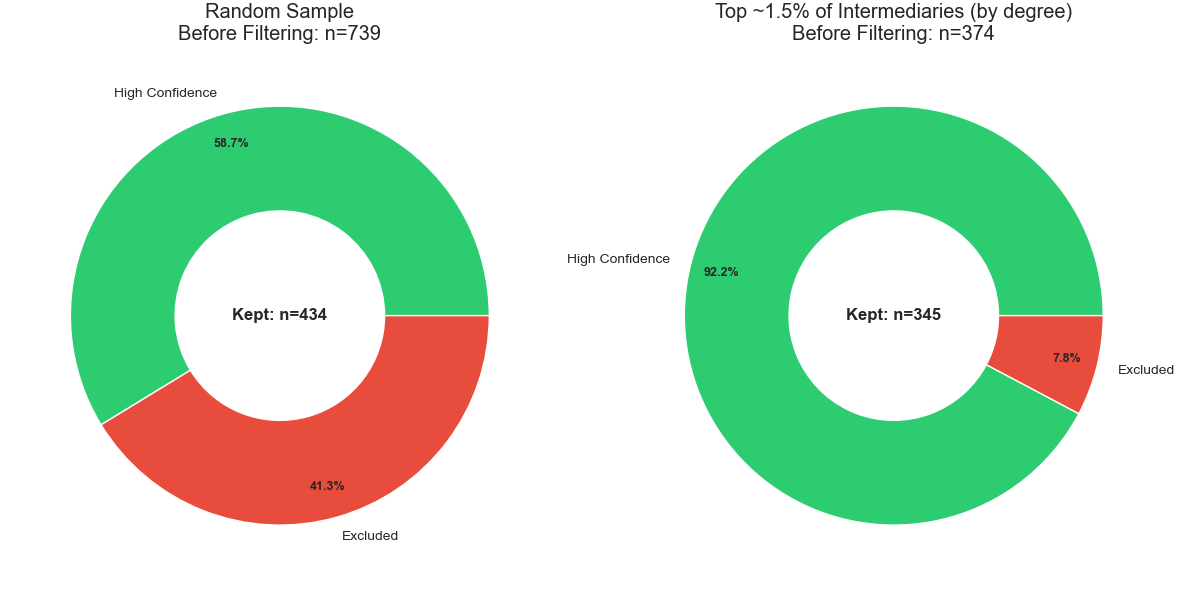
\includegraphics[width=0.8\textwidth]{Appendix_Filtering_of_Enrichment.png}
    \caption{Filtering Process of the Samples for Function-Classification}
    \label{fig:appendix_filtering_enrichment}
\end{figure}

\newpage

\section{(More) Geography and Jurisdiction Heatmaps for Intermediaries at Country-Level}

\begin{figure}[htbp]
    \centering
    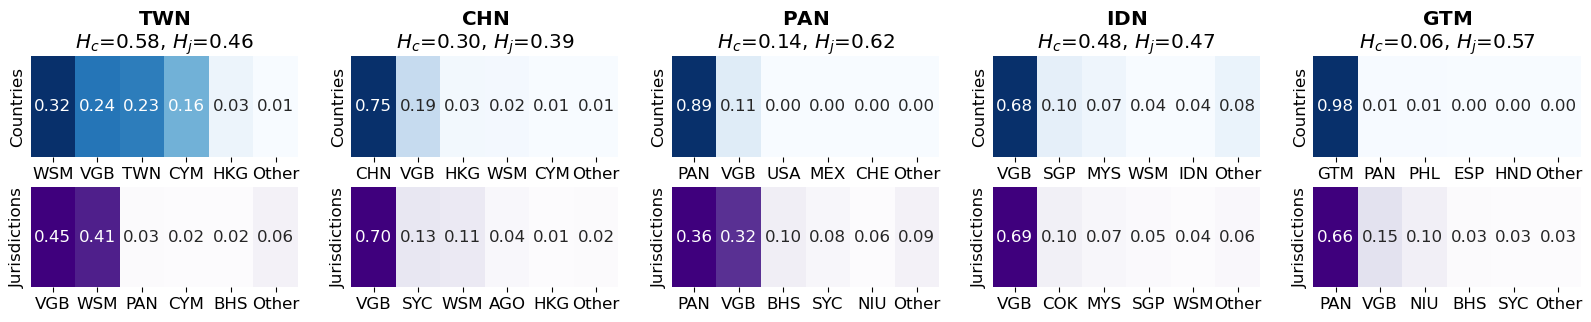
\includegraphics[width=0.9\textwidth]{images/Geography_Country_Heatmaps_Top6_10.png}
    \caption{Client and Incorporation Jurisdiction Heatmap for Intermediaries in Top 6-10 Countries (TWN, CHN, PAN, IDN, GTM)}
    \label{fig:geography_country_heatmaps_top6_10}
\end{figure}
\begin{figure}[htbp]
    \centering
    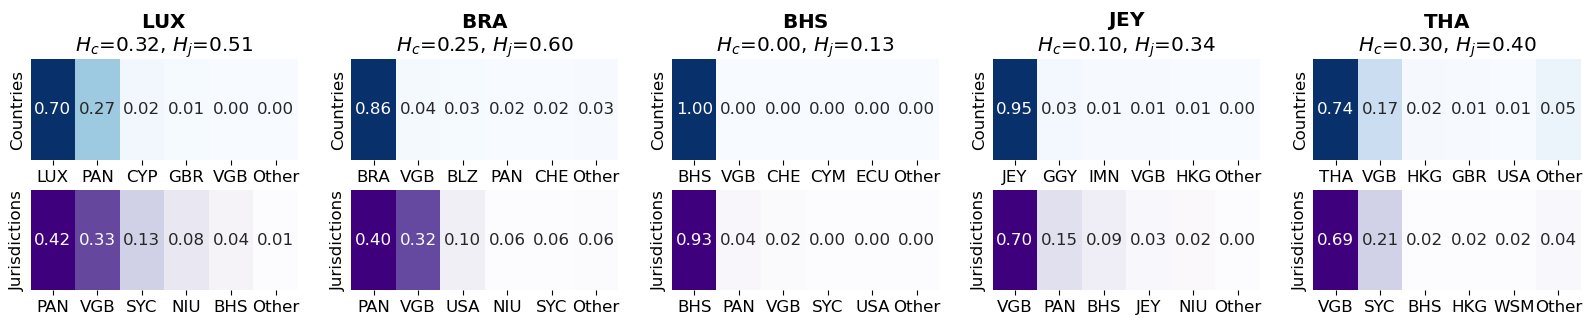
\includegraphics[width=0.9\textwidth]{images/Geography_Country_Heatmaps_Top11_15.png}
    \caption{Client and Incorporation Jurisdiction Heatmap for Intermediaries in Top 11-15 Countries (LUX, BRA, BHS, JEY, THA)}
    \label{fig:geography_country_heatmaps_top11_15}
\end{figure}

\textbf{Figures \ref{fig:geography_country_heatmaps_top6_10} and \ref{fig:geography_country_heatmaps_top11_15} – Intermediaries in Top 6-15 Countries:}
These figures reveal patterns for other significant intermediary locations, including emerging economies and traditional OFCs.

\begin{itemize}
    \item \textbf{China (CHN)} (Figure \ref{fig:geography_country_heatmaps_top6_10}): Similar to Hong Kong, shows a strong domestic client focus (CHN, 75\%; $H_c=0.30$) and a preference for VGB (70\%) and Samoa (WSM, 13\%) for incorporations ($H_j=0.39$).

    \item \textbf{Panama (PAN)} (Figure \ref{fig:geography_country_heatmaps_top6_10}): As a major OFC itself, Panamanian intermediaries overwhelmingly serve entities active in Panama (PAN, 89\%; $H_c=0.14$). They primarily use their own jurisdiction for incorporation (PAN, 36\%), but also VGB (32\%) and USA (10\%), leading to higher jurisdictional diversity ($H_j=0.62$). This suggests a role in both domestic incorporation and facilitating access to other OFCs for local clients.

    \item \textbf{Luxembourg (LUX)} (Figure \ref{fig:geography_country_heatmaps_top11_15}): Another key European financial center, Luxembourg-based intermediaries primarily serve domestic clients (LUX, 70\%; $H_c=0.32$). Their incorporation choices are relatively diverse ($H_j=0.51$), favoring Panama (PAN, 42\%), VGB (33\%), and Seychelles (SYC, 13\%).

    \item \textbf{Bahamas (BHS)} (Figure \ref{fig:geography_country_heatmaps_top11_15}): Shows an extreme domestic client focus (BHS, 100\%; $H_c=0.00$), with intermediaries almost exclusively using the Bahamas itself for incorporation (BHS, 93\%; $H_j=0.13$). This points to a highly localized service model within the OFC.

    \item \textbf{Jersey (JEY)} (Figure \ref{fig:geography_country_heatmaps_top11_15}): Intermediaries in this Crown Dependency also exhibit a very strong domestic client focus (JEY, 93\%; $H_c=0.10$) and primarily use VGB (70\%) for incorporations ($H_j=0.34$).
\end{itemize}

An illustrative example of specific geographical specialization is provided by Cyprus-based intermediaries (Figure \ref{fig:geography_country_heatmaps_cyprus}). Cyprus is well-documented in academic and policy literature for its strong financial links to Russia (e.g., Alstadsæter et al., 2022, note similar patterns for Dubai facilitating Russian wealth). While Russia is generally underrepresented as a client country in the broader ICIJ dataset for intermediaries from most other nations, entities serviced by Cypriot intermediaries show a significant Russian presence. As seen in the top bar of Figure \ref{fig:geography_country_heatmaps_cyprus}, 12\% of entities serviced by Cypriot intermediaries are linked to activity in Russia (RUS). This proportion is notably higher than Russia's typical share in the client portfolios of intermediaries from the other top 15 countries (often negligible or grouped under "Other"), suggesting a strong, specific association—a high "lift" in association analysis terms—for the Cyprus-Russia connection. Beyond Russia, Cypriot intermediaries primarily serve entities active in Cyprus itself (CYP, 34\%), the United Arab Emirates (ARE, 27\%), and, interestingly, the British Virgin Islands (VGB, 26\%). The VGB share here might reflect entities whose ultimate beneficial owners or complex operational activities are channeled through or managed from VGB, rather than VGB being a primary country of economic activity in the traditional sense. For incorporations (bottom bar), Cypriot intermediaries heavily favor VGB (56\%), followed by Seychelles (SYC, 15\%), the Bahamas (BHS, 15\%), and Panama (PAN, 9\%). The entropy values for Cyprus-based intermediaries ($H_c = 0.55, H_j = 0.53$) are both above the median values observed in Figure \ref{fig:geography_country_level_entropy_distribution}, indicating a moderately diversified client base and a similarly moderate diversification in their choice of incorporation jurisdictions, despite the prominent Russian nexus.

\begin{figure}[htbp]
    \centering
    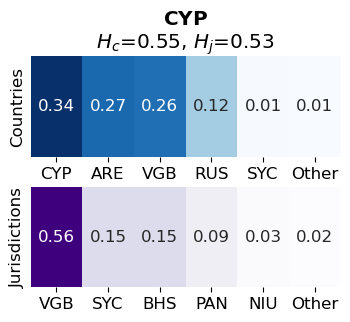
\includegraphics[width=0.5\textwidth]{images/Geography_Country_Heatmaps_Cyprus.png} % Adjusted width for single panel
    \caption{Client and Incorporation Jurisdiction Heatmap for Cyprus-based Intermediaries}
    \label{fig:geography_country_heatmaps_cyprus}
\end{figure}

\newpage

\section{Degree Distribution of Intermediaries}

\label{subsubsec:degree_dist_intermediaries}
A recurring theme in the study of complex networks, and one that underpins much of the analytical framework of this thesis, is the prevalence of power-law-like distributions in various network metrics. This characteristic is particularly evident in the degree distribution of intermediaries within the ICIJ dataset, as illustrated in Figure \ref{fig:preliminary_powerlaw_fit}. This is an established finding in the literature (e.g. Chang et al., 2023a), however, it is replicated here because of its importance for the thesis - and also serves as an indirect robustness check for the data. We essentially reproduce their finding, though the overlaw power-law estimates arrived at are different compared to Chang et al. (2023a) who find even fatter tails in the subset of countries (USA, Hong Kong, China, and Russia) they analyze. They land on an exponent of $\alpha \approx 1.2-1.4$ for the degree distribution of intermediaries in their sample, while we find $\alpha \approx 2.08$ for the full dataset. 

\begin{figure}[htbp]
    \centering
    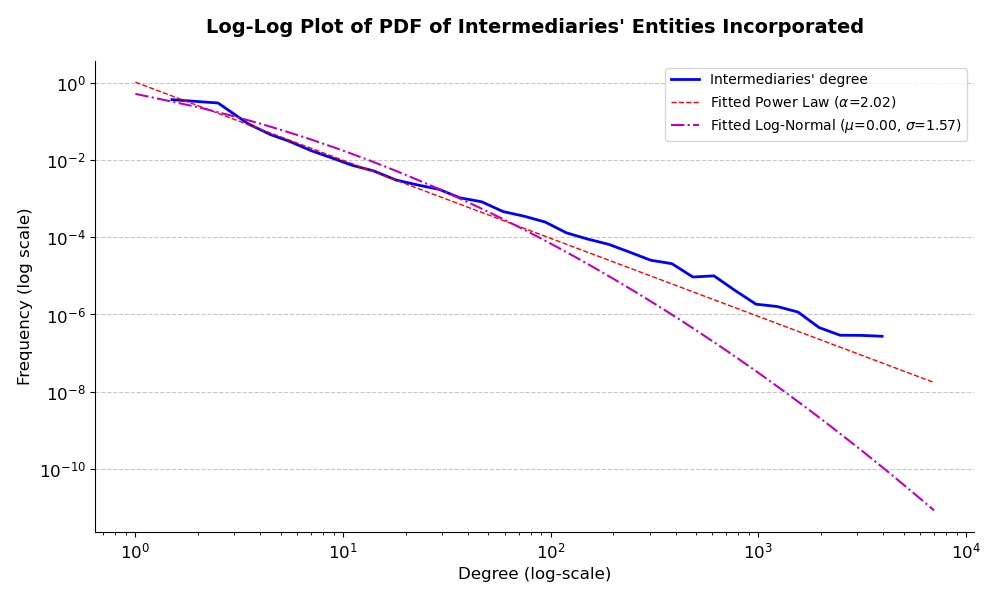
\includegraphics[width=0.8\textwidth]{images/Preliminary_Powerlaw_Fit.png} % Assuming images are in an 'images' subdirectory
    \caption{Degree Distribution of Intermediaries and Model Fits}
    \label{fig:preliminary_powerlaw_fit}
\end{figure}

Figure \ref{fig:preliminary_powerlaw_fit} plots the probability density function (PDF) of intermediary degrees on a log-log scale. This type of scaling is standard for visualizing heavy-tailed distributions, as a true power law will appear as a straight line. The empirical data (blue line) clearly shows a long tail, indicating that while the vast majority of intermediaries are connected to a relatively small number of entities, a few intermediaries possess an extraordinarily high number of connections. These are the "super-hubs" of the offshore world, intermediaries that facilitate the creation and administration of thousands, or even tens of thousands, of offshore entities. This visual observation aligns with findings from structural studies of similar large-scale datasets, such as Kejriwal and Dang's (2020) network analysis of the Panama Papers (a subset of the ICIJ data, we are working with), which also identified power-law degree distributions for actors within that leak. Such a distribution points to a highly heterogeneous system where certain intermediaries play a disproportionately significant role in structuring offshore financial networks.

To formally assess the nature of this distribution, the fit of a power-law model was compared to that of a log-normal distribution, a common alternative for heavy-tailed data. A log-likelihood ratio test yielded $R = 57.0287$ with a $p$-value $< 0.0001$. This result provides strong statistical evidence that a power-law model offers a significantly better fit to the empirical intermediary degree distribution than a log-normal model, or at the very least, confirms that the distribution is distinctly heavy-tailed. The fitted power-law distribution (red dashed line in Figure \ref{fig:preliminary_powerlaw_fit}) has an exponent $\alpha \approx 2.08$. In scale-free networks, $\alpha$ typically falls between 2 and 3; a value closer to 2, as observed here, signifies a particularly "fat" tail, indicating an even more pronounced dominance of the largest hubs compared to networks with higher $\alpha$ values. The log-normal fit (purple dash-dot line), by contrast, visibly underestimates the probability of observing these extremely high-degree intermediaries.

The implications of this scale-free or heavy-tailed characteristic are profound for understanding the architecture and dynamics of the offshore financial system. It suggests a system that is not randomly organized but has an inherent structure where a few key intermediaries may act as critical "enablers" or "chokepoints" (Chang et al., 2023b; Christensen, 2024). The existence of these super-hubs implies that a significant portion of offshore activity is channeled through a limited number of actors. This concentration has several potential consequences:
\begin{itemize}
    \item \textbf{Efficiency and Scalability:} These hubs may provide economies of scale, making it easier and more efficient to create and manage large numbers of offshore entities.
    \item \textbf{Vulnerability:} As demonstrated by Chang et al. (2023b) in their study of oligarch networks, systems with such scale-free properties are often robust to the random removal of nodes but critically vulnerable to the targeted disruption of their main hubs. This suggests that regulatory or law enforcement actions focused on these key intermediaries could have a disproportionately large impact on the overall network.
    \item \textbf{Influence and Diffusion:} Highly connected intermediaries could be pivotal in disseminating specific tax planning strategies, financial products, or even compliance norms throughout the network.
\end{itemize}

\newpage

\section{Proposition 3: Structural Centrality of Microstates in Intermediation Network}

The hardest part has been to leave so much material on the cutting-floor. I've, however, not had the willpower to completely relinquish this section of my thesis, and so with the brazen immaturity of a Bachelor's student, I've put it here, in the vain hope that the efforts won't feel wasted. 

I here propose a third proposition. Briefly stated, it posits a core set of Offshore Financial Centers (OFCs), that is central in the jurisdictions and countries that intermediaries \textit{co-service}. This is to be understood as, whenever that intermediaries do business in multiple countries, the countries they take advantage of are these microstates; that these OFCs constitute "anonymous" jurisdiction and countries, cosmopolitan and therefore not tied to any specific client base, but rather a global clientele. This is in contrast to the "local anchors" of intermediaries, which are often tied to specific client bases, and therefore more likely to be found in larger countries.

This may also be due to their offering of versatile ``legal technologies'' like ``Dual-Purpose'' vehicles as for example is proposed in Laffitte (2024). Empirical confirmation that they form the structural backbone of the global offshore network, and are countries that intermediaries from all countries whose residents they do business and jurisdiction they incorporate. Critical hubs and bridges in chains of intermediation, facilitating complex offshore strategies regardless of client or intermediary home country. Looking at the central actors in these networks of countries that intermediaries make use of. This is where network analysis shines, with its cohsive langauge of ``centrality'' and ``community detection''.

There are three main facts in support of this proposition, that will be covered later in the appendix.
\begin{itemize}
    \item High centrality (betweenness, eigenvector) of jurisdictions like VGB, BHS, PAN, CYM, HKG in your co-service and co-usage networks.
    \item Dominance of ``Dual-Purpose'' legal technologies in the central core of the jurisdiction co-usage network.
    \item High lift values between key OFCs in association analysis.
\end{itemize}

This section proceeds in "reverse order", first having described the overall proposition, and then the methods.

\subsection{Concepts from Network Analysis}
\label{subsec:network_theory_concepts}

Specifically, network analysis is employed here to uncover the roles intermediaries play based on their positions within the interconnected offshore financial system revealed by the ICIJ data. As described in Section \ref{sec:3_1}, the ICIJ data forms a multi-modal graph (comprising entities, officers, intermediaries, etc.). Directly applying many standard network analysis concepts to such a multipartite graph can be challenging. Therefore, our approach often involves analyzing specific projections or subsets of the global graph to make the analytical tools from network theory applicable. The foundational textbook by Newman (2010) serves as the primary reference for this section.

\begin{itemize}
    \item \textbf{Centrality Scores}: To identify nodes of critical importance within specific network representations, we utilize two fundamental centrality measures. In the context of understanding the key countries for intermediary activity, these measures are applied to a network derived from intermediary incorporation patterns.
    \begin{itemize}
        \item \textbf{Eigenvector Centrality}: This measure assigns scores to nodes based on the principle that connections to high-scoring nodes contribute more to the score of the node in question than equal connections to low-scoring nodes. It is calculated as the principal eigenvector of the adjacency matrix $\mathbf{A}$ of the network, satisfying $x_i = \frac{1}{\lambda} \sum_{j} A_{ij} x_j$, where $x_i$ is the centrality score of node $i$, $A_{ij}$ is 1 if node $i$ is connected to node $j$ and 0 otherwise (or the weight of the edge), and $\lambda$ is the largest eigenvalue of $\mathbf{A}$ (cf. Perron-Frobenius theorem). Eigenvector centrality is chosen for its ability to identify nodes that are influential not just by having many connections, but by being connected to other influential nodes, providing a robust reading of which countries are most central in the network of intermediary incorporations.
        \item \textbf{Betweenness Centrality}: This metric quantifies the extent to which a node lies on shortest paths between other pairs of nodes. For a node $v$, it is defined as $C_B(v) = \sum_{s \neq v \neq t} \frac{\sigma_{st}(v)}{\sigma_{st}}$, where $\sigma_{st}$ is the total number of shortest paths between nodes $s$ and $t$, and $\sigma_{st}(v)$ is the number of those paths that pass through $v$. Betweenness centrality is used here to gauge which countries act as crucial "bridges" or conduits within the network, potentially connecting otherwise disparate segments, a role distinct from simply being a high-degree hub.
    \end{itemize}

    \item \textbf{Community Detection: Modularity Maximization}: To uncover clusters or communities of closely related nodes within the country network, we employ modularity maximization. This approach provides an atheoretical method for identifying densely connected groups of countries, which may reflect underlying similarities in how intermediaries utilize them. Such clustering could be influenced by factors like shared regime types (Chang et al., 2023c) or the trust dynamics inherent in relational capitalism. While traditional clustering algorithms could be applied, defining a meaningful distance or dissimilarity metric for nodes in these networks is non-trivial. Modularity maximization, conversely, assesses the quality of a partition by comparing the number of intra-community edges to what would be expected in a random network with similar properties (a null model). The quality of a partition $C$ is measured by the modularity $Q$:
    \begin{equation}
        Q = \frac{1}{2m} \sum_{i,j} \left[ A_{ij} - P_{ij} \right] \delta(c_i, c_j)
    \end{equation}
    where $m$ is the total number of edges, $A_{ij}$ is the actual weight of the edge between nodes $i$ and $j$, $P_{ij}$ is the expected weight of an edge between $i$ and $j$ under the Newman-Girvan null model (a configuration model preserving the degree sequence, where $P_{ij} = \frac{k_i k_j}{2m}$ for unweighted graphs, $k_i$ being the degree of node $i$), and $\delta(c_i, c_j)$ is 1 if nodes $i$ and $j$ are in the same community ($c_i=c_j$) and 0 otherwise. Since finding the optimal partition is an NP-hard (although, to be honest, at the size we reduce our graph sizes, search space isn't an issue...) problem, we utilize the Louvain method (Blondel et al., 2008), an efficient and widely adopted greedy algorithm, as implemented in the \texttt{networkx} library.

    \item \textbf{Power-law Distribution}: The distribution of node degrees (number of connections) and other network properties are examined for characteristics of power-law distributions. A power law, $P(k) \sim k^{-\alpha}$, describes a "fat-tailed" distribution where a few nodes (hubs) have a disproportionately high number of connections, while most nodes have few. Such distributions are frequently observed in real-world networks (Clauset et al., 2009; Kejriwal \& Dang, 2020) and their presence can indicate significant heterogeneity in node importance.

    \item \textbf{Density of a Graph}: Network density, the ratio of actual edges to the total number of possible edges in the network ($D = \frac{L}{N(N-1)/2}$ for an undirected graph with $L$ edges and $N$ nodes), is used to measure the general level of connectedness. Low density is typical for large, sparse networks and indicates that connections are selective rather than ubiquitous.
\end{itemize}

\subsection{Association Analysis}
\label{subsec:unsupervised_learning}
In line with the highly exploratory nature of this thesis, unsupervised learning techniques are employed to discover notable patterns within the data. Association analysis (Hastie et al., 2009) is particularly opportune for identifying non-obvious relationships or co-occurrences in large datasets, such as the ICIJ networks. For example, it can help determine which connections (e.g., between a type of intermediary and the use of a specific jurisdiction or legal technology) are particularly remarkable. This approach relies on a \textbf{non-parametric notion} of pattern discovery, aiming to \textbf{discover patterns of high density} or co-occurrence.

Two main tools from association analysis, based on simple set-theoretical notions, are used:
\begin{itemize}
    \item \textbf{Support}: This measures the overall frequency of an itemset (e.g., a specific attribute or combination of attributes) in the dataset. For an itemset $X$, $Support(X) = P(X) = \frac{\text{count}(X)}{N}$, where $N$ is the total number of transactions (e.g., intermediaries). For an association rule $A \rightarrow B$, $Support(A \rightarrow B) = P(A \cup B)$.
    \item \textbf{Lift}: This measures how much more likely item $B$ is to be present when item $A$ is present, compared to the baseline probability of $B$. It indicates the strength of an association beyond what would be expected by chance.
    \begin{equation}
        Lift(A \rightarrow B) = \frac{P(B|A)}{P(B)} = \frac{Support(A \cup B)}{Support(A) \times Support(B)}
    \end{equation}
    A lift value greater than 1 suggests a positive association, a value less than 1 suggests a negative association, and a value of 1 suggests independence. \textbf{Lift scores} will be used to quantify the strength of associations found, indicating, for example, how much more likely an intermediary of a certain type is to use a specific jurisdiction compared to the overall likelihood.
\end{itemize}

\subsection{Patterns of Co-Specialisation}
To explore these co-service relationships further, a network of countries was constructed. In this network, countries are nodes, and an edge exists between two countries if at least one intermediary serves clients (entities) linked to both. The weight of the edge reflects the number of distinct intermediaries serving clients in both countries. The resulting full country network consists of 121 nodes (countries) and 2,716 edges. Key summary statistics for this network are presented in Table \ref{tab:country_network_summary}. 

\begin{table}[htbp]
\centering
\caption{Summary Statistics for the Full Country Co-Service Network}
\label{tab:country_network_summary}
\begin{tabular}{lc}
\toprule
\textbf{Metric}                        & \textbf{Value}    \\
\midrule
Number of Nodes               & 121      \\
Number of Edges               & 2716     \\
Network Density               & 0.3741   \\
Average Degree                & 44.89    \\
Average Clustering Coefficient & 0.7728   \\
\bottomrule
\end{tabular}
\end{table}

Visualising such dense graphs is incredibly challenging. Therefore, to identify the most important connections, the network was filtered using principles from association analysis. Edges are displayed only if they 1) meet a minimum support threshold (representing at least 0.008 of all intermediaries' country-pair connections, meaning the pair is co-serviced by at least that fraction of intermediaries who service multiple countries) and 2) a lift score of 1.5 or higher. Lift measures how much more frequently two countries are co-serviced than would be expected if their servicing by intermediaries were independent. This filtering ensures that the visualized connections are not only reasonably frequent but also represent associations significantly stronger than chance, that they are both common links as well as carrying statistical signal. The resulting filtered network, or "backbone," thus highlights the most robust and significant co-service relationships. While the exact number of nodes included is sensitive to the choice of the lift and support thresholds here, this "backbone" as I term it, is relatively stable across a range of thresholds.

The nodes in the network visualization (Figure \ref{fig:geography_cross_country_network}) are coloured in two ways: first, by communities identified using the Louvain modularity maximization algorithm (Blondel et al., 2008), which groups densely interconnected countries; and second, by regime type using VDem data, as described in Section \ref{sec:3_2}. This dual coloring was intended to explore whether regime type influences intermediary operations and co-service patterns, a factor suggested by literature on offshore secrecy strategies (e.g. Chang et al., 2023b).

\begin{figure}[htbp]
    \centering
    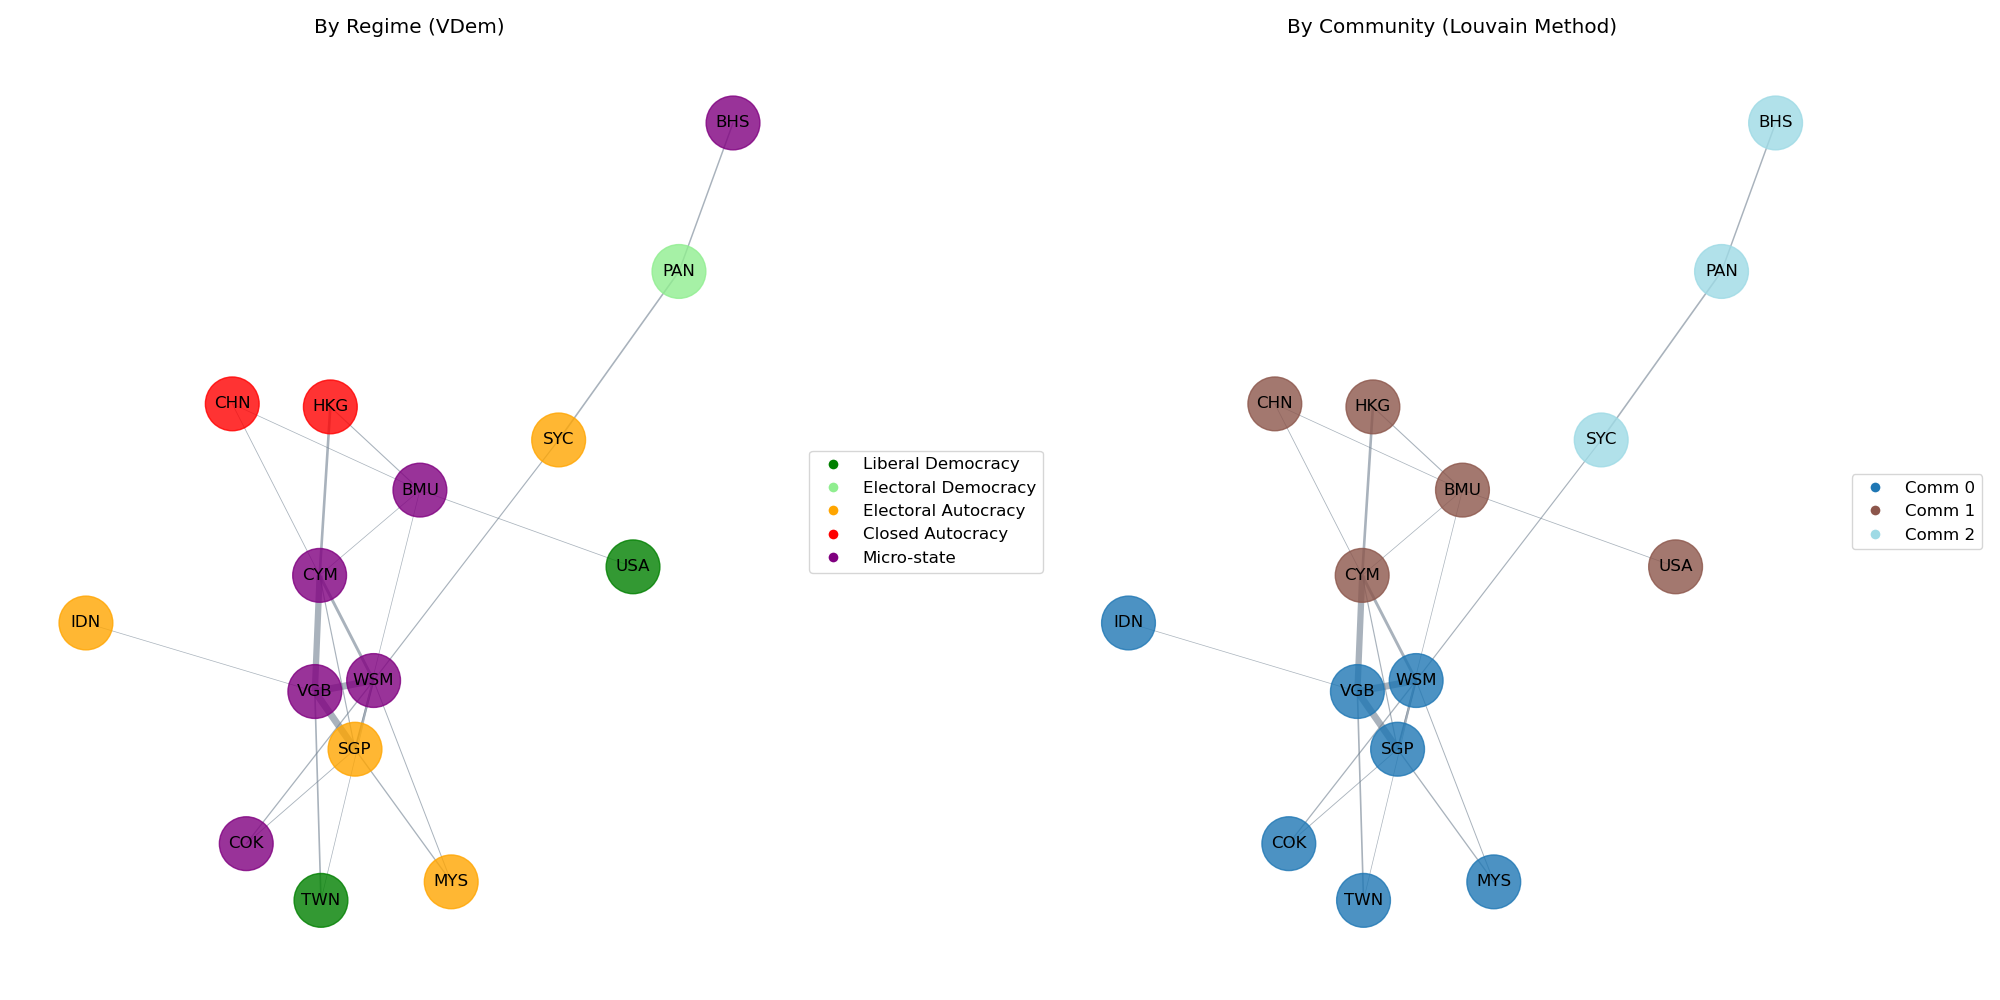
\includegraphics[width=0.9\textwidth]{Geography_Cross_Country_Network.png}
    \caption{Filtered Network of Co-Served Countries, Coloured by Louvain Community (left) and Regime Type (right). Edges shown have support $\ge 0.008$ and lift $\ge 1.5$}
    \label{fig:geography_cross_country_network}
\end{figure}

\subsection{Interpretation of the Filtered Country Network Structure}
The filtered network (Figure \ref{fig:geography_cross_country_network}) reveals a sparse yet highly structured set of relationships, forming a distinct core-periphery structure. A central core of interconnected nodes is evident, particularly involving VGB (British Virgin Islands), CYM (Cayman Islands), and SGP (Singapore), along with their strong links to HKG (Hong Kong) and BMU (Bermuda).

When coloured by regime type, no clear large-scale clustering emerges that aligns strictly with political systems. The central cluster itself is diverse, including Micro-states (VGB, CYM, BMU), jurisdictions classified as Closed Autocracies (HKG, reflecting its unique status), and Electoral Autocracies (SGP). Liberal Democracies such as the USA and TWN (Taiwan) are present but connect to nodes of various different regime types. This visual evidence supports the notion that regime type, while potentially a factor in individual elite choices (Chang et al., 2023c), is not a primary driver of these strong, systemic co-service relationships at the country-network level. Economic roles, historical ties, and financial infrastructure likely play more dominant roles in shaping this backbone.

The Louvain community detection method, which is data-driven, reveals distinct groupings based on the density of co-service links:
\begin{itemize}
    \item \textbf{Community 0 (Dark Blue):} This is the largest community, featuring prominent offshore centers like VGB and CYM, major Asian economies/financial hubs like SGP, TWN (Taiwan), MYS (Malaysia), IDN (Indonesia), and Pacific jurisdictions like COK (Cook Islands) and likely WSM (Samoa, if present in the filtered graph). This highlights strong ties between several offshore financial centers and key Asian economies.
    \item \textbf{Community 1 (Brown):} This community comprises major economies like the USA and CHN (China), alongside HKG (Hong Kong) and the offshore jurisdiction BMU (Bermuda), indicating a distinct Atlantic-Pacific nexus involving Bermuda.
    \item \textbf{Community 2 (Light Blue):} A smaller, distinct community consisting of PAN (Panama), SYC (Seychelles), and BHS (Bahamas), all of which are significant offshore jurisdictions.
\end{itemize}
Most nodes in this backbone network are connected within two to three steps, indicating a relatively compact structure despite the filtering.

Centrality metrics calculated on the full 121-node co-service network (detailed in Appendix Tables \ref{tab:appendix_country_betweenness_app} and \ref{tab:appendix_country_eigenvector_app}) identify key players.
\textbf{VGB (British Virgin Islands)} is dominant, exhibiting the highest betweenness and eigenvector centrality, underscoring its pivotal role in connecting diverse client countries through shared intermediaries. The \textbf{USA} ranks second in both measures, reflecting its economic importance and the global reach of its client base serviced by international intermediaries. The USA is linked to BMU (Bermuda) in the filtered graph's Community 1. \textbf{HKG (Hong Kong) \& CHN (China)} also feature prominently in centrality scores and are central to Community 1. Numerous \textbf{Micro-states} (BMU, BHS, CYM) show high centrality, consistent with their specialized roles in offshore finance. \textbf{SGP (Singapore)} is another key, highly central node, bridging various parts of the network. In general, high centrality in the full network translates to a significant structural role in this filtered backbone, indicating that the most connected countries in the overall system also form the core of the strongest co-service relationships.

\subsection{Significant Country Associations}

Lift scores from the association analysis (top associations detailed in Appendix Table \ref{tab:appendix_significant_country_associations_app}, filtered for co-occurrences $\ge 20$) reveal particularly strong and statistically significant pairings, many of which are visualized in Figure \ref{fig:geography_cross_country_network} (those with lift $\ge 1.5$).
Key findings include:
\begin{itemize}
    \item Strong \textbf{Micro-state synergies} are evident. For instance, the WSM-CYM (Samoa-Cayman Islands) pairing shows a high lift of 6.78, and VGB-CYM (British Virgin Islands-Cayman Islands) has a lift of 1.91. These indicate that intermediaries servicing clients in one of these micro-states are substantially more likely to also service clients in the other, suggesting complementary service offerings or established pathways for specific client types. The CYM-BMU (Cayman Islands-Bermuda) link is exceptionally strong with a lift of 13.5.
    \item A critical \textbf{China-Bermuda nexus} emerges with CHN-BMU showing a very high lift of 15.3. This suggests Bermuda acts as a particularly favored intermediary hub for clients linked to China. This is complemented by the USA-BMU link (lift 4.92), highlighting Bermuda's role in Community 1 of the filtered network, connecting major economic powers.
    \item Robust \textbf{Asian connections} are underscored by pairs like SGP-MYS (Singapore-Malaysia, lift 5.27). Singapore (SGP) also shows strong co-service patterns with various Micro-states such as WSM (Samoa, lift 3.04) and CYM (Cayman Islands, lift 3.89), reinforcing its role as a key hub in Community 0.
    \item A distinct \textbf{PAN-SYC-BHS nexus} (Community 2) is confirmed with pairings like PAN-SYC (Panama-Seychelles) having a lift of 3.89.
    \item Crucially, high lift values are common \textbf{across different regime types}. For example, China (Closed Autocracy) has a very high lift with Bermuda (Micro-state), and the USA (Liberal Democracy) also has a significant lift with Bermuda. This reinforces the earlier observation that factors beyond regime similarity, such as specialized financial services, established legal and commercial pathways, or historical ties, are potent drivers of these strong co-service relationships.
\end{itemize}

\subsubsection{Network of Jurisdictions Used by Intermediaries}
\label{subsubsec:network_jurisdictions_used}

Shifting focus from client locations to incorporation locations, this section analyzes the network of jurisdictions that intermediaries use in combination. The full jurisdiction co-usage network, where an edge exists if an intermediary incorporates entities in both jurisdictions (weighted by the number of such intermediaries), comprises 41 nodes and 347 edges. Summary statistics are provided in Table \ref{tab:jurisdiction_network_summary}. The distribution of the number of distinct jurisdictions used per intermediary is shown in Figure \ref{fig:geography_distribution_jurisdictions_by_intermediary}, indicating that most intermediaries utilize a small portfolio of jurisdictions, though some use many.

\begin{table}[htbp]
\centering
\caption{Summary Statistics for the Full Jurisdiction Co-Service Network}
\label{tab:jurisdiction_network_summary}
\begin{tabular}{lc}
\toprule
\textbf{Metric}                        & \textbf{Value}    \\
\midrule
Number of Nodes               & 41       \\
Number of Edges               & 347      \\
Network Density               & 0.4232   \\
Average Degree                & 16.93    \\
Average Clustering Coefficient & 0.8155   \\
\bottomrule
\end{tabular}
\end{table}

Figure \ref{fig:geography_cross_jurisdiction_network} presents a filtered "backbone" of these co-usage patterns, applying the same support ($\ge 0.008$) and lift ($\ge 1.5$) thresholds as for the country co-service network. Nodes are coloured by their predominant legal technology profile (derived from Laffitte, 2024, as detailed in Section \ref{sec:3_2}) and by Louvain communities. The image displays the most prominent nodes in this filtered network, including CRI (Costa Rica), SGP (Singapore), CYP (Cyprus), GBR (Great Britain), BLZ (Belize), AGO (Angola), HKG (Hong Kong), CYM (Cayman Islands), COK (Cook Islands), MYS (Malaysia), BHS (Bahamas), SYC (Seychelles), PAN (Panama), NIU (Niue), WSM (Samoa), and USA.

\begin{figure}[htbp]
    \centering
    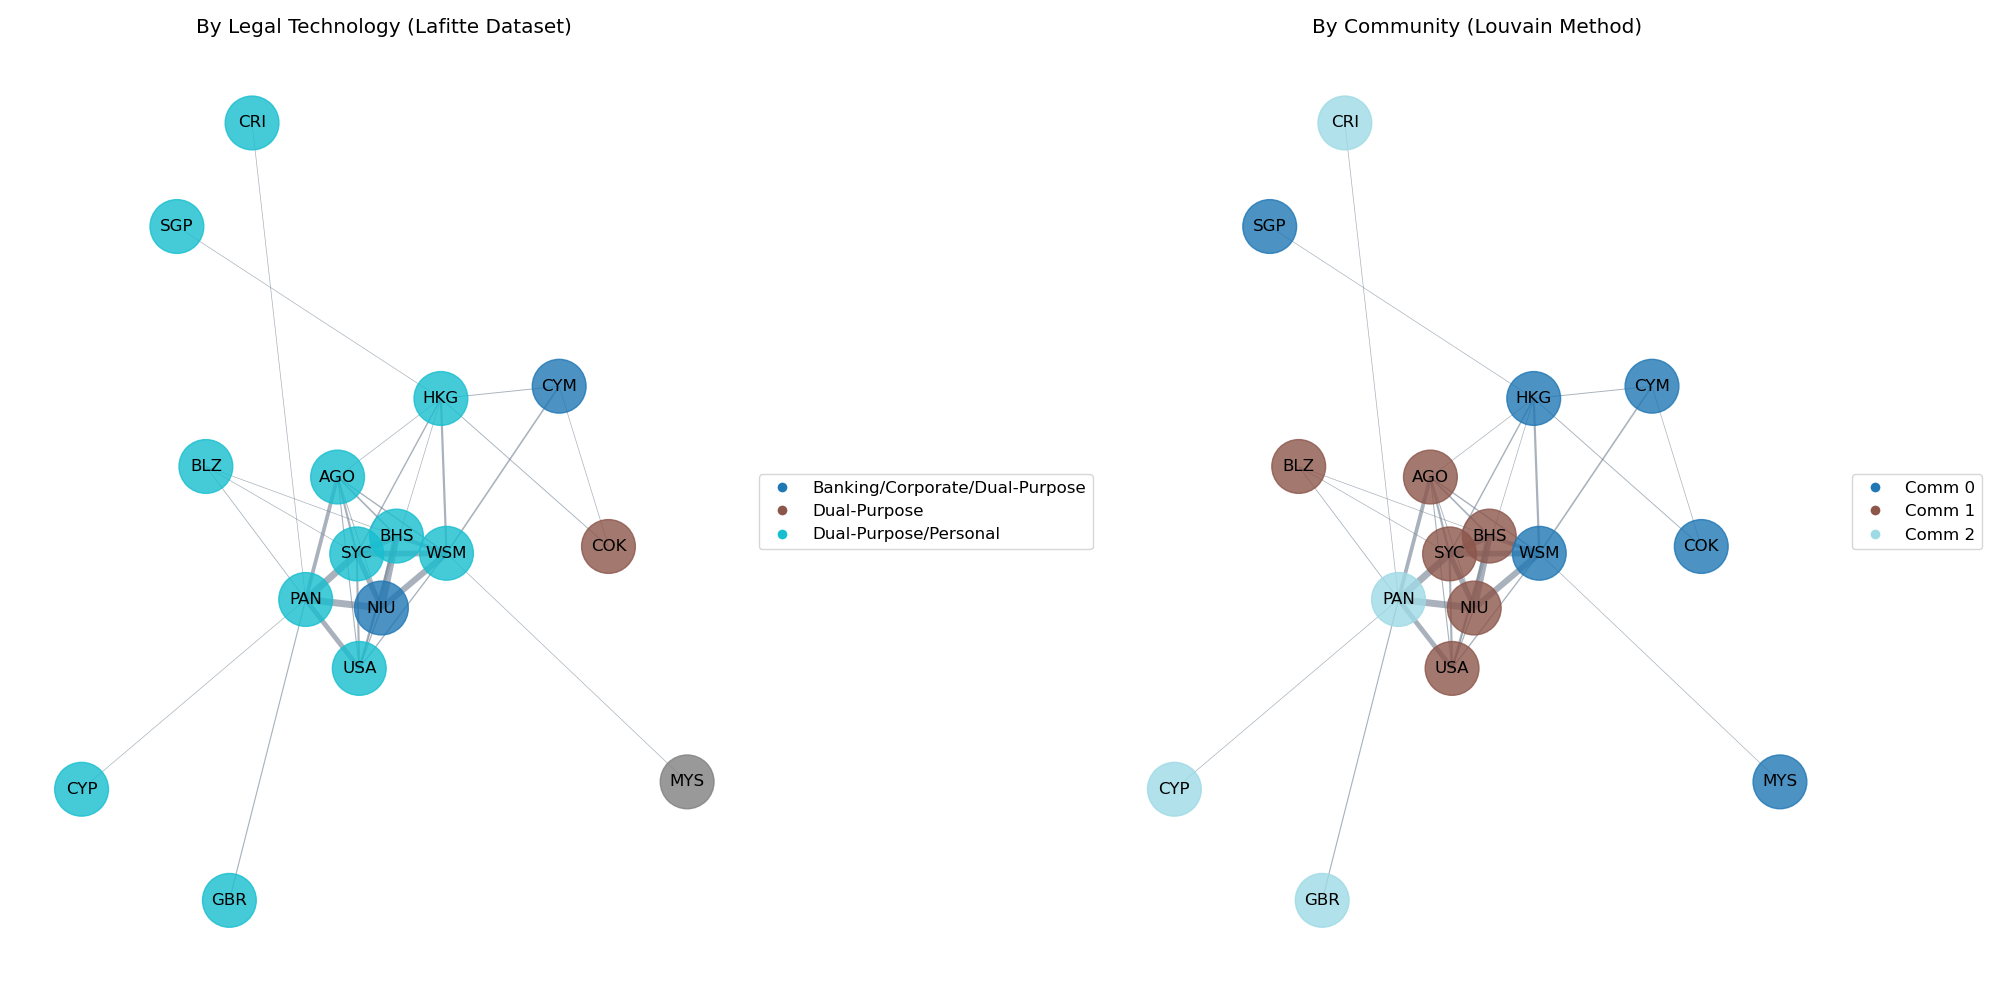
\includegraphics[width=0.9\textwidth]{Geography_Cross_Jurisdiction_Network.png}
    \caption{Filtered Network of Co-Used Jurisdictions, Coloured by Legal Technology (left) and Louvain Community (right). Edges shown have support $\ge 0.008$ and lift $\ge 1.5$.}
    \label{fig:geography_cross_jurisdiction_network}
\end{figure}

\subsection{Interpretation of the Filtered Jurisdiction Network Structure}
The filtered jurisdiction network (Figure \ref{fig:geography_cross_jurisdiction_network}) reveals a central, densely connected core. Key jurisdictions in this core include BHS (Bahamas), SYC (Seychelles), AGO (Angola), WSM (Samoa), NIU (Niue), PAN (Panama), USA, and HKG (Hong Kong).

When coloured by their predominant legal technology profile (Laffitte, 2024), the central cluster is overwhelmingly dominated by jurisdictions offering \textbf{"Dual-Purpose"} legal technologies (e.g., International Business Companies - IBCs). This strongly supports the observation that central jurisdictions in this co-usage network are those providing flexible, widely applicable corporate vehicles suitable for both corporate and personal wealth structuring. 

Louvain community detection identifies the following groupings based on co-usage patterns:
\begin{itemize}
    \item \textbf{Community 1 (Brown):} This is the largest and most central community, encompassing jurisdictions like USA, PAN, NIU, BHS, SYC, AGO, and WSM. These are largely characterized by "Dual-Purpose" legal technologies.
    \item \textbf{Community 0 (Dark Blue):} This community includes HKG, CYM (Cayman Islands), and COK (Cook Islands), combining jurisdictions known for "Banking/Corporate/Dual-Purpose" (like HKG) with those strong in "Dual-Purpose/Personal" (like CYM, COK).
    \item \textbf{Community 2 (Light Blue):} This community is more peripheral in the filtered network and includes SGP (Singapore), CRI (Costa Rica), CYP (Cyprus), GBR (Great Britain), BLZ (Belize), and MYS (Malaysia), representing a mix of financial centers and specialized offshore jurisdictions.
\end{itemize}

\subsection{Centrality in the Jurisdiction Network}
Centrality metrics for the full 41-jurisdiction co-usage network (detailed in Appendix Tables \ref{tab:appendix_jurisdiction_betweenness_app} and \ref{tab:appendix_jurisdiction_eigenvector_app}) are revealing.
\textbf{VGB (British Virgin Islands)} ranks first in both betweenness and eigenvector centrality in the full network, confirming its paramount importance as an incorporation jurisdiction. However, it is strikingly absent from the filtered graph in Figure \ref{fig:geography_cross_jurisdiction_network}. This implies that while VGB is co-used with many other jurisdictions by numerous intermediaries, these individual pairings might not meet the specific high support and lift thresholds chosen for this backbone view (requiring at least 20 co-occurrences and lift $\ge 1.5$). This suggests VGB's role might be more as a general-purpose, widely connected jurisdiction whose strong pairings are numerous but perhaps more diffuse, rather than concentrated in extremely high-lift niche combinations that also meet the co-occurrence threshold.
\textbf{BHS (Bahamas)} and \textbf{PAN (Panama)} rank second and third, respectively, in overall centrality and are visibly central within the filtered graph, particularly in Community 1. \textbf{HKG (Hong Kong)} and \textbf{CYM (Cayman Islands)} are also highly central in the full network and form a core part of Community 0 in the filtered view. Most other top-ranked jurisdictions by centrality align with their prominence in the backbone, with VGB being the main exception due to the filtering criteria.

\subsection{Significant Jurisdiction Associations}
Association analysis, focusing on lift scores from statistically significant pairs with at least 20 co-occurrences (detailed in Appendix Table \ref{tab:appendix_significant_jurisdiction_associations_app}), highlights robust co-usage patterns:
\begin{itemize}
    \item The dominant \textbf{Community 1 (largely "Dual-Purpose" hubs)} shows very high mutual lift values. For instance, BHS-NIU (Bahamas-Niue) has a lift of 4.6 (support 0.016), and NIU-WSM (Niue-Samoa) has a lift of 5.3 (support 0.012). NIU (Niue) appears as a critical connector within this cluster of Pacific and Caribbean jurisdictions, also showing strong lift with SYC (Seychelles, lift 4.1, support 0.010).
    \item \textbf{Community 0 (financial centers and specialized OFCs)}: The HKG-CYM (Hong Kong-Cayman Islands) pairing shows a strong lift of 5.8 (support 0.0018), indicating a significant tendency for intermediaries using one to also use the other. WSM-CYM (Samoa-Cayman Islands) also shows a notable lift of 4.6 (support 0.0031).
    \item Strong co-usage is observed between jurisdictions offering \textbf{similar legal technology profiles}. For example, many of the high-lift pairs within Community 1 involve jurisdictions predominantly offering "Dual-Purpose" or "Dual-Purpose/Personal" technologies.
\end{itemize}


\subsection{Country Network Centrality and Associations}
\label{sec:appendix_country_network}

Table \ref{tab:appendix_country_betweenness_app} lists the top 10 countries by betweenness centrality and Table \ref{tab:appendix_country_eigenvector_app} by eigenvector centrality in the full co-service network. Table \ref{tab:appendix_significant_country_associations_app} details significant country associations.

\begin{table}[htbp]
\centering
\caption{Top 10 Countries by Betweenness Centrality in the Full Co-Service Network}
\label{tab:appendix_country_betweenness_app}
\begin{tabular}{lrrrr}
\toprule
Node & Betweenness & Eigenvalue & Appearances & Regime              \\
\midrule
VGB  & 0.18    & 0.14    & 6285        & Micro-state         \\
USA  & 0.053    & 0.13    & 1042        & Liberal Democracy   \\
CHE  & 0.039    & 0.13    & 1545        & Liberal Democracy   \\
GBR  & 0.028    & 0.13    & 1258        & Liberal Democracy   \\
MUS  & 0.024    & 0.13    & 139         & Liberal Democracy   \\
BHS  & 0.021    & 0.13    & 489         & Micro-state         \\
BMU  & 0.020    & 0.13    & 103         & Micro-state         \\
PAN  & 0.020    & 0.096    & 1203        & Electoral Democracy \\
SGP  & 0.019    & 0.13    & 578         & Electoral Autocracy \\
URY  & 0.017    & 0.031    & 318         & Liberal Democracy   \\
\bottomrule
\end{tabular}
\end{table}

\begin{table}[htbp]
\centering
\caption{Top 10 Countries by Eigenvector Centrality in the Full Co-Service Network}
\label{tab:appendix_country_eigenvector_app}
\begin{tabular}{lrrrr}
\toprule
Node & Eigenvalue & Betweenness & Appearances & Regime              \\
\midrule
VGB  & 0.14    & 0.18    & 6285        & Micro-state         \\
USA  & 0.13    & 0.053    & 1042        & Liberal Democracy   \\
GBR  & 0.13    & 0.028    & 1258        & Liberal Democracy   \\
HKG  & 0.13    & 0.016    & 2865        & Closed Autocracy    \\
JEY  & 0.13    & 0.013    & 390         & Micro-state         \\
CHN  & 0.13    & 0.0085    & 320         & Closed Autocracy    \\
CAN  & 0.13    & 0.0088    & 195         & Liberal Democracy   \\
BHS  & 0.13    & 0.021    & 489         & Micro-state         \\
SGP  & 0.13    & 0.019    & 578         & Electoral Autocracy \\
CYM  & 0.13    & 0.012    & 363         & Micro-state         \\
\bottomrule
\end{tabular}
\end{table}

\clearpage
{\scriptsize % Smaller font for the large table
\begin{longtable}{@{}lllp{2.2cm}p{2.2cm}rrr@{}}
\caption{Significant Country Associations in Co-Service Network (Bonferroni Corrected $p < 6.89 \times 10^{-6}$)} \\
\label{tab:appendix_significant_country_associations_app} \\
\toprule
    & u   & v   & u\_regime            & v\_regime            & support  & lift      & p\_value      \\
\midrule
\endfirsthead
\multicolumn{8}{c}%
{{\tablename\ \thetable{} -- continued from previous page}} \\
\toprule
    & u   & v   & u\_regime            & v\_regime            & support  & lift      & p\_value      \\
\midrule
\endhead
\midrule
\multicolumn{8}{r}{{Continued on next page}} \\
\midrule
\endfoot
\bottomrule
\endlastfoot
76  & VGB & WSM & Micro-state         & Micro-state         & 0.017    & 1.87      & 7.24e-46  \\
498 & WSM & CYM & Micro-state         & Micro-state         & 0.0035   & 6.78      & 1.34e-45  \\
105 & VGB & CYM & Micro-state         & Micro-state         & 0.0076   & 1.91      & 9.58e-23  \\
775 & CHN & BMU & Closed Autocracy    & Micro-state         & 0.00088  & 15.3      & 3.36e-19  \\
2405& CYM & BMU & Micro-state         & Micro-state         & 0.00088  & 13.5      & 4.46e-18  \\
2032& SGP & MYS & Electoral Autocracy & Electoral Autocracy & 0.0016   & 5.27      & 5.66e-17  \\
102 & VGB & SGP & Micro-state         & Electoral Autocracy & 0.010    & 1.60      & 9.75e-17  \\
351 & PAN & SYC & Electoral Democracy & Electoral Autocracy & 0.0020   & 3.89      & 8.08e-16  \\
501 & WSM & COK & Micro-state         & Micro-state         & 0.0015   & 4.84      & 1.57e-15  \\
496 & WSM & SGP & Micro-state         & Electoral Autocracy & 0.0025   & 3.04      & 1.89e-14  \\
2044& SGP & BMU & Electoral Autocracy & Micro-state         & 0.00083  & 8.06      & 5.07e-13  \\
488 & WSM & SYC & Micro-state         & Electoral Autocracy & 0.0014   & 4.14      & 2.36e-12  \\
2033& SGP & CYM & Electoral Autocracy & Micro-state         & 0.0014   & 3.89      & 1.75e-11  \\
2035& SGP & COK & Electoral Autocracy & Micro-state         & 0.0010   & 4.63      & 2.23e-10  \\
1190& USA & BMU & Liberal Democracy   & Micro-state         & 0.00092  & 4.92      & 4.62e-10  \\
497 & WSM & TWN & Micro-state         & Liberal Democracy   & 0.00083  & 5.48      & 5.27e-10  \\
768 & CHN & CYM & Closed Autocracy    & Micro-state         & 0.00096  & 4.75      & 8.31e-10  \\
2034& SGP & MUS & Electoral Autocracy & Liberal Democracy   & 0.00071  & 5.07      & 4.46e-08  \\
419 & JEY & BMU & Micro-state         & Micro-state         & 0.00050  & 7.16      & 1.17e-07  \\
642 & HKG & CYM & Closed Autocracy    & Micro-state         & 0.0032   & 1.75      & 6.61e-07  \\
650 & HKG & BMU & Closed Autocracy    & Micro-state         & 0.0013   & 2.52      & 6.83e-07  \\
502 & WSM & MYS & Micro-state         & Electoral Autocracy & 0.0012   & 2.75      & 1.54e-06  \\
2039& SGP & TWN & Electoral Autocracy & Liberal Democracy   & 0.00054  & 5.04      & 1.85e-06  \\
2307& AUS & IRL & Liberal Democracy   & Liberal Democracy   & 0.00021  & 22.0      & 3.25e-06  \\
\end{longtable}
} 
\clearpage
\newpage


\subsection{Jurisdiction Network Centrality and Associations}
\label{sec:appendix_jurisdiction_network}

Table \ref{tab:appendix_jurisdiction_betweenness_app} shows the top 10 jurisdictions by betweenness centrality and Table \ref{tab:appendix_jurisdiction_eigenvector_app} by eigenvector centrality in the full co-usage network. Significant jurisdiction associations are detailed in Table \ref{tab:appendix_significant_jurisdiction_associations_app}.

\begin{table}[htbp]
\centering
\caption{Top 10 Jurisdictions by Betweenness Centrality in the Full Co-Service Network}
\label{tab:appendix_jurisdiction_betweenness_app}
\resizebox{\textwidth}{!}{%
\begin{tabular}{@{}lrrrl@{}}
\toprule
Node & Betweenness & Eigenvalue & Appearances & Jurisdiction Legal Technology                               \\
\midrule
VGB  & 0.20    & 0.26    & 13533       & Dual-Purpose/Personal                                       \\
BHS  & 0.084    & 0.26    & 2099        & Banking/Corporate/Dual-Purpose/Other Technologies/Personal  \\
PAN  & 0.060    & 0.25    & 6533        & Banking/Corporate/Dual-Purpose                              \\
HKG  & 0.058    & 0.24    & 625         & Banking/Corporate/Other Technologies                        \\
CYM  & 0.048    & 0.21    & 290         & Banking/Corporate/Dual-Purpose                              \\
WSM  & 0.027    & 0.20    & 1352        & Dual-Purpose/Personal                                       \\
USA  & 0.019    & 0.23    & 387         & None                                                        \\
COK  & 0.018    & 0.12    & 954         & Banking/Corporate/Dual-Purpose/Personal                     \\
CYP  & 0.017    & 0.22    & 45          & Banking/Corporate/Dual-Purpose                              \\
SGP  & 0.013    & 0.19    & 355         & Banking/Other Technologies                                  \\
\bottomrule
\end{tabular}
}
\end{table}

\begin{table}[htbp]
\centering
\caption{Top 10 Jurisdictions by Eigenvector Centrality in the Full Co-Service Network}
\label{tab:appendix_jurisdiction_eigenvector_app}
\resizebox{\textwidth}{!}{%
\begin{tabular}{@{}lrrrl@{}}
\toprule
Node & Eigenvalue & Betweenness & Appearances & Jurisdiction Legal Technology                               \\
\midrule
VGB  & 0.26    & 0.20    & 13533       & Dual-Purpose/Personal                                       \\
BHS  & 0.26    & 0.084    & 2099        & Banking/Corporate/Dual-Purpose/Other Technologies/Personal  \\
PAN  & 0.25    & 0.060    & 6533        & Banking/Corporate/Dual-Purpose                              \\
HKG  & 0.24    & 0.058    & 625         & Banking/Corporate/Other Technologies                        \\
USA  & 0.23    & 0.019    & 387         & None                                                        \\
CYP  & 0.22    & 0.017    & 45          & Banking/Corporate/Dual-Purpose                              \\
CYM  & 0.21    & 0.048    & 290         & Banking/Corporate/Dual-Purpose                              \\
WSM  & 0.20    & 0.027    & 1352        & Dual-Purpose/Personal                                       \\
JEY  & 0.20    & 0.011    & 28          & Dual-Purpose/Other Technologies                             \\
SGP  & 0.19    & 0.013    & 355         & Banking/Other Technologies                                  \\
\bottomrule
\end{tabular}
}
\end{table}

\clearpage
{\tiny % Even smaller font for this very wide table
\begin{longtable}{@{}lllp{3cm}p{3cm}rrr@{}} % Adjusted column spec and count
\caption{Significant Jurisdiction Associations in Co-Service Network (Bonferroni Corrected $p < 6.10 \times 10^{-5}$)} \\
\label{tab:appendix_significant_jurisdiction_associations_app} \\
\toprule
    & u   & v   & u\_legal\_technology                             & v\_legal\_technology                             & support  & lift      & p\_value      \\ % Removed weight and odds_ratio
\midrule
\endfirsthead
\multicolumn{8}{c}% % Adjusted column span
{{\tablename\ \thetable{} -- continued from previous page}} \\
\toprule
    & u   & v   & u\_jurisdiction\_legal\_technology                             & v\_jurisdiction\_legal\_technology                             & support  & lift      & p\_value      \\ % Removed weight and odds_ratio
\midrule
\endhead
\midrule
\multicolumn{8}{r}{{Continued on next page}} \\ % Adjusted column span
\midrule
\endfoot
\midrule
\bottomrule
\endlastfoot
72  & BHS & NIU & Bnk/Corp/Dual/Oth Tech/Pers & Dual-Purpose                & 0.016    & 4.6       & 1.80e-165 \\
108 & NIU & WSM & Dual-Purpose                & Dual-Purpose/Personal       & 0.012    & 5.3       & 9.68e-134 \\
106 & NIU & SYC & Dual-Purpose                & Dual-Purpose/Personal       & 0.010    & 4.1       & 1.89e-85  \\
122 & SYC & WSM & Dual-Purpose/Personal       & Dual-Purpose/Personal       & 0.011    & 3.3       & 4.50e-73  \\
3   & PAN & SYC & Bnk/Corp/Dual-Purpose       & Dual-Purpose/Personal       & 0.027    & 1.6       & 2.50e-49  \\
73  & BHS & SYC & Bnk/Corp/Dual/Oth Tech/Pers & Dual-Purpose/Personal       & 0.013    & 2.3       & 2.62e-48  \\
123 & SYC & AGO & Dual-Purpose/Personal       & None                        & 0.0043   & 4.6       & 2.20e-40  \\
4   & PAN & USA & Bnk/Corp/Dual-Purpose       & None                        & 0.0095   & 2.2       & 1.33e-39  \\
121 & SYC & USA & Dual-Purpose/Personal       & None                        & 0.0041   & 4.2       & 9.61e-36  \\
143 & USA & AGO & None                        & None                        & 0.0021   & 8.6       & 1.49e-32  \\
2   & PAN & NIU & Bnk/Corp/Dual-Purpose       & Dual-Purpose                & 0.018    & 1.6       & 1.88e-32  \\
174 & WSM & CYM & Dual-Purpose/Personal       & Bnk/Corp/Dual-Purpose       & 0.0031   & 4.6       & 1.31e-29  \\
1   & PAN & BHS & Bnk/Corp/Dual-Purpose       & Bnk/Corp/Dual/Oth Tech/Pers & 0.033    & 1.4       & 3.87e-29  \\
74  & BHS & USA & Bnk/Corp/Dual/Oth Tech/Pers & None                        & 0.0042   & 3.0       & 1.33e-23  \\
162 & WSM & HKG & Dual-Purpose/Personal       & Bnk/Corp/Oth Tech           & 0.0043   & 2.9       & 4.59e-23  \\
204 & HKG & CYM & Bnk/Corp/Oth Tech           & Bnk/Corp/Dual-Purpose       & 0.0018   & 5.8       & 3.16e-21  \\
107 & NIU & USA & Dual-Purpose                & None                        & 0.0025   & 3.9       & 1.05e-19  \\
6   & PAN & AGO & Bnk/Corp/Dual-Purpose       & None                        & 0.0074   & 1.8       & 3.80e-18  \\
163 & WSM & AGO & Dual-Purpose/Personal       & None                        & 0.0027   & 3.2       & 1.30e-16  \\
140 & USA & WSM & None                        & Dual-Purpose/Personal       & 0.0026   & 2.8       & 8.95e-14  \\
7   & PAN & GBR & Bnk/Corp/Dual-Purpose       & None                        & 0.0023   & 2.4       & 1.50e-13  \\
76  & BHS & AGO & Bnk/Corp/Dual/Oth Tech/Pers & None                        & 0.0032   & 2.4       & 3.06e-13  \\
128 & SYC & BLZ & Dual-Purpose/Personal       & Bnk/Corp/Dual-Purpose/Pers  & 0.00092  & 6.0       & 3.06e-12  \\
75  & BHS & WSM & Bnk/Corp/Dual/Oth Tech/Pers & Dual-Purpose/Personal       & 0.0080   & 1.6       & 3.94e-12  \\
10  & PAN & CRI & Bnk/Corp/Dual-Purpose       & None                        & 0.0011   & 3.1       & 7.44e-11  \\
109 & NIU & AGO & Dual-Purpose                & None                        & 0.0017   & 2.8       & 2.41e-09  \\
81  & BHS & BLZ & Bnk/Corp/Dual/Oth Tech/Pers & Bnk/Corp/Dual-Purpose/Pers  & 0.00083  & 3.7       & 1.18e-07  \\
34  & VGB & NIU & Dual-Purpose/Personal       & Dual-Purpose                & 0.025    & 1.1       & 4.69e-07  \\
9   & PAN & CYP & Bnk/Corp/Dual-Purpose       & Bnk/Corp/Dual-Purpose       & 0.0012   & 2.3       & 9.42e-07  \\
207 & HKG & SGP & Bnk/Corp/Oth Tech           & Bnk/Oth Tech                & 0.0011   & 2.8       & 2.53e-06  \\
125 & SYC & HKG & Dual-Purpose/Personal       & Bnk/Corp/Oth Tech           & 0.0028   & 1.8       & 3.98e-06  \\
\end{longtable}
} % End tiny
\clearpage






